\documentclass{article}
\usepackage[utf8]{inputenc}
\usepackage{dirtree}
\usepackage{graphicx}
\graphicspath{ {./images/}}
\title{data description}
\author{chomans }
\date{October 2018}

\begin{document}

\section{Data Structure}
The \texttt{climate\_data} directory's file structure is generally simple: we have a collection of directories corresponding to climate models, and within each climate model's directory a collection of \texttt{.nc} and .mat files corresponding to climate variables. For the purposes of our visualization, we are interested in the \texttt{.nc} files.

See below for a directory structure diagram, showing how our data are organized with respect to the climate model which generated them. Note that we only show partial lists of files and directories of interest -- the entire directory is quite large, and contains many files, including several strays that can safely be ignored. That is, for several sample climate models, we give lists of several \texttt{.nc} files representative of the kinds of variables contained within the directory. The next section contains a description of the meaning of the filenames for data stored in \texttt{.nc} format.

\medskip
\dirtree{%
.1 /project/moyer/climate\_data.
.2 README.txt.
.2 CCSM3.
.3 pr\_Amon\_CCSM3\_abrupt8x\_LongRunMIP\_000101-145012.nc.
.3 psl\_Amon\_CCSM3\_abrupt2x\_LongRunMIP\_000101-300012.nc.
.3 rlut\_Amon\_CCSM3\_abrupt2x\_LongRunMIP\_000101-300012.nc.
.3 tos\_yrr\_CCSM3\_control\_LongRunMIP\_1-1530.nc.
.3 ....
.2 CCSM4.
.3 huss\_day\_CCSM4\_rcp85\_r6i1p1\_20760101-21001231.nc.
.3 pr\_Amon\_CCSM4\_historical\_r6i1p1\_185001-200512.nc.
.3 psl\_day\_CCSM4\_historical\_r6i1p1\_19500101-19891231.nc.
.3 tas\_Amon\_CCSM4\_piControl\_r2i1p1\_095301-110812.nc.
.3 ....
.2 ACCESS1-3.
.3 cl\_Amon\_ACCESS1-3\_historical\_r1i1p1\_195001-197412.nc.
.3 clt\_day\_ACCESS1-3\_historical\_r1i1p1\_19750101-19991231.nc.
.3 ua\_day\_ACCESS1-3\_historical\_r1i1p1\_19750101-19791231.nc.
.3 ....
.2 CESM1-0-4.
.2 CMORPH.
.2 ECEARTH.
.2 ERA-INTERIM.
.2 FAMOUS.
.2 LongRunMIP.
.2 ....
}\medskip

As this directory is located on Midway, data can be copied to local machines with your tool of choice, e.g. SCP or Globus. For example, if you wished to use the (nonexistent) "\texttt{example.nc}" file generated with the equally nonexistent "\texttt{EXAMPLE}" climate model, you could simply type the following into the command line:\\ 


\texttt{scp [user]@midway1.rcc.uchicago.edu:/project/moyer/climate\_data/EXAMPLE/example.nc /[desired]/[local]/[location]}

\section{Sample Files for Visualization}
A small sample set of files which the tool must be able to visualize, together covering potential stumbling blocks. Taken together, these files cover each possible temporal resolution, as well as the largest and smallest grid resolution, we seek to visualize, as well as cases where special considerations for visualization are required. All files are within the \texttt{/project/moyer/climate\_data/} directory.

\begin{enumerate}
    \item \texttt{/CanESM2/ua\_day\_CanESM2\_historical\_r1i1p1\_19410101-19501231.nc} \\
          \texttt{/CanESM2/va\_day\_CanESM2\_historical\_r1i1p1\_19410101-19501231.nc} \\
          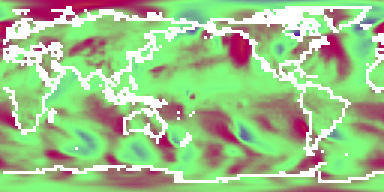
\includegraphics[scale = 0.4]{va}
          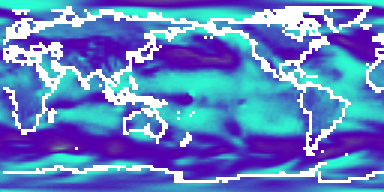
\includegraphics[scale = 0.4]{ua}
          
          These two files represent, respectively, the eastward and northward wind speed on each day between 1941/01/01 and 1950/12/31, in the CanESM2 model. Their grid resolution is 128x64: this is the smallest resolution we seek to visualize. They should be visualized together to generate wind speed vectors for animation. Units: $m/s$.
          
    \item \texttt{/CCSM4/pr\_Amon\_CCSM4\_historical\_r6i1p1\_185001-200512.nc} \\
    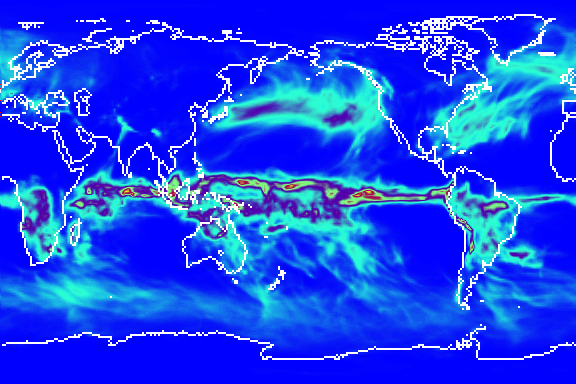
\includegraphics[width=11cm, height=6cm]{pr_amon_ccsm4_historical_r6i1p1_185001-200512}
    
    This file represents the precipitation amount for every month between January 1850 and December 2005, in the CCSM4 model. Its grid resolution is 288x192, the largest resolution we seek to visualize. No special considerations are required for visualizing it. Units: $kg m^{-2} s^{-1}$.
    
    \item \texttt{/CCSM4/pr\_Amon\_CCSM4\_historical\_r6i1p1\_185001-200512.nc} \\
    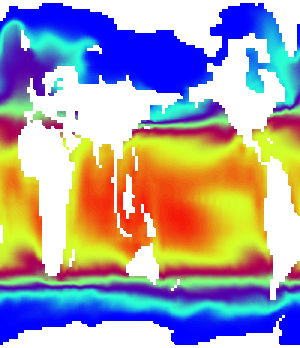
\includegraphics[width=11cm, height=6cm]{ss}
    
    This file represents the ocean surface temperature for every year between 1 CE and 3000 CE, in the CanESM2 model. Its grid resolution is 100x116. Note that the variable is only defined where ocean is found. Units: degrees Celsius.
          		
\end{enumerate}
\section{Further Information on the NetCDF format, Climate Variables and Visualization}

We are interested in visualization of NetCDF files, which store numerical data arranged as arrays of variables, where each entry in an array has corresponding entires in special arrays called dimensions, representing, for example, time, latitude, or longitude. RDCEP stores NetCDF files with the extension \texttt{.nc}. The vast majority of our \texttt{.nc} files contain one climate-related variable. These variables can be many things: for example, they may represent surface temperature, quantity of precipitation, or component vectors for wind speed. This variable of interest is encoded within the file as a function of latitude (\texttt{lat}), longitude (\texttt{lon}), and time (\texttt{time}). Sometimes, height from surface is another dimension, and sometimes height is fixed in a given file (if this is the case, it is usually documented in the filename). This encoding is extremely useful for our purposes because of the nature of our planned visualization: one variable whose values at different points
on the globe are represented as color, evolving with time in the animation.

Filenames follow the format described here, courtesy Kevin Schwarzwald:
\begin{verbatim}
[var]_[freq]_[model]_[experiment]_[ensemble (member)]_[time range]_[suffix] 

- [var]: file variable shorthand, based on CMIP5 definitions wherever
possible (i.e. "tas" for near-surface air temperature)
- [freq]: interval between time-samples (i.e. "day" or "ann")
- [model]: the name of the model (i.e. "MIROC-ESM")
- [experiment]: the relevant experiment, for example a forcing
scenario (i.e. "rcp85")
- [ensemble (member)]: an identification of the ensemble member; for
CMIP5 models, this is a set formula of "r#i#p#", showing run,
iteration, and microphysics, respectively. For non-CMIP5 models, this can be
any other identifier of the run, as long as it doesn't use "." or "_" in its
description
- [time range]: in [yyyy(mm(dd))]-[yyyy(mm(dd))] format
- [suffix]: optional suffix; for example "_DATA" for processed data
\end{verbatim}
Here is a list of variable shorthand for some variables of interest for the visualization (these are variables that we already can visualize with the modified nullschool tool). Note both that NetCDF files encode units and the full name of the variable (in metadata). To get a sense of the contents of any \texttt{.nc} file, you can use the open-source \texttt{ncview} (which also produces images) or \texttt{ncdump} Unix tools.
\begin{itemize}
    \item \texttt{tas} - Temperature At Surface ($K$)
    \item \texttt{psl} - Pressure, Sea Level ($\frac{N}{m^2}$)
    \item \texttt{pr} - Precipitation ($\frac{kg}{m^{2} s}$)
    \item \texttt{ua} - Wind speed, u-component($\frac{m}{s}$)
    \item \texttt{va} - Wind speed, v-component($\frac{m}{s}$)
\end{itemize}

A further note about wind speed: it is encoded as two separate variables, but the nullschool approach, and
probably the best, is to encode the magnitude of the two component’s sum as the color scale and indicate
the direction through the motion of a particle layer over the static vector field.

Many other variables exist in the \texttt{climate\_data} directory. We can easily develop schema to visualize many of them, as the format corresponds exactly to the visualization, but such schema do not yet exist.
\end{document}
